\documentclass[12pt]{article}
\usepackage[utf8]{inputenc}
\usepackage[spanish]{babel}
\decimalpoint
\usepackage{amsmath}
\usepackage{caption}
\usepackage{amsthm}
\usepackage{amssymb}
\usepackage{graphicx}
\usepackage[margin=0.9in]{geometry}
\usepackage{fancyhdr}
\usepackage[inline]{enumitem}
\usepackage{float}
\usepackage{cancel}
\usepackage{bigints}
\usepackage{color}
\usepackage{xcolor}
\usepackage{listingsutf8}
\usepackage{algorithm}
\usepackage{tocloft}
\usepackage[none]{hyphenat}
\usepackage{graphicx}
\usepackage{grffile}
\usepackage{tabularx}
\usepackage[nottoc,notlot,notlof]{tocbibind}
\usepackage{times}
\usepackage{color}
\definecolor{gray97}{gray}{.97}
\definecolor{gray75}{gray}{.75}
\definecolor{gray45}{gray}{.45}
\renewcommand{\cftsecleader}{\cftdotfill{\cftdotsep}}
\pagestyle{fancy}
\setlength{\headheight}{15pt} 
\lhead{EJERCICIO 7 - Diseño de soluciones PD}
\rhead{\thepage}
\lfoot{ESCOM-IPN}
\renewcommand{\footrulewidth}{0.5pt}
\setlength{\parskip}{0.5em}
\newcommand{\ve}[1]{\overrightarrow{#1}}
\newcommand{\abs}[1]{\left\lvert #1 \right\lvert}
\date{26 de febrero de 2017}
\title{Pruebas a posteriori}
\author{Reporte 1}

\definecolor{pblue}{rgb}{0.13,0.13,1}
\definecolor{pgreen}{rgb}{0,0.5,0}
\definecolor{pred}{rgb}{0.9,0,0}
\definecolor{pgrey}{rgb}{0.46,0.45,0.48}
\lstset{tabsize=1}

\usepackage{listings}
\lstset{ frame=Ltb,
framerule=0pt,
aboveskip=0.5cm,
framextopmargin=3pt,
framexbottommargin=3pt,
framexleftmargin=0.4cm,
framesep=0pt,
rulesep=.4pt,
backgroundcolor=\color{gray97},
rulesepcolor=\color{black},
%
stringstyle=\ttfamily,
showstringspaces = false,
basicstyle=\small\ttfamily,
commentstyle=\color{gray45},
keywordstyle=\bfseries,
%
numbers=left,
numbersep=15pt,
numberstyle=\tiny,
numberfirstline = false,
breaklines=true,
}

% minimizar fragmentado de listados
\lstnewenvironment{listing}[1][]
{\lstset{#1}\pagebreak[0]}{\pagebreak[0]}

\lstdefinestyle{consola}
{basicstyle=\scriptsize\bf\ttfamily,
backgroundcolor=\color{gray75},
}

\lstdefinestyle{Java}
{language=Java,
}

%%%%%%%%%%%%%%%%%%%%%

\lstdefinestyle{customc}{
  belowcaptionskip=1\baselineskip,
  breaklines=true,
  frame=L,
  xleftmargin=\parindent,
  language=C,
  showstringspaces=false,
  basicstyle=\footnotesize\ttfamily,
  keywordstyle=\bfseries\color{green!40!black},
  commentstyle=\itshape\color{purple!40!black},
  identifierstyle=\color{blue},
  stringstyle=\color{orange},
}

\lstdefinestyle{customasm}{
  belowcaptionskip=1\baselineskip,
  frame=L,
  xleftmargin=\parindent,
  language=[x86masm]Assembler,
  basicstyle=\footnotesize\ttfamily,
  commentstyle=\itshape\color{purple!40!black},
}

\lstset{escapechar=@,style=customc}


    % =====  CODE EDITOR =========
    \lstdefinestyle{CompilandoStyle} {                              %This is Code Style
        backgroundcolor=\color{BlueGrey800MD},                      %Background Color  
        basicstyle=\tiny\color{white},                              %Font color
        commentstyle=\color{BlueGrey100MD},                         %Comment color
        stringstyle=\color{TealMD},                                 %String color
        keywordstyle=\color{Green100MD},                            %keywords color
        numberstyle=\tiny\color{TealMD},                            %Size of a number
        frame=shadowbox,                                            %Adds a frame around the code
        breakatwhitespace=true,                                     %Style                       
        breaklines=true,                                            %Style                   
        keepspaces=true,                                            %Style                   
        numbers=left,                                               %Style                   
        numbersep=10pt,                                             %Style 
        xleftmargin=\parindent,                                     %Style 
        tabsize=4                                                   %Style 
    }
 
    \lstset{style=CompilandoStyle}                                  %Use this style

    \usepackage{minted} % Paquete que permite citar codigo
    \usemintedstyle{borland} % Aqui se define el colorscheme para minted
    \setminted{
        fontsize = \scriptsize, % Ajusta el codigo a la hoja
        baselinestretch = 1,
        linenos, % set numbers
        breaklines=true, % Hace un salto de linea automatico en caso de que se llege al final de la line
        tabsize=3 
    }

%Permite crear columnas en el documento
\usepackage{multicol} 
\usepackage{color}
\usepackage{comment}
\newcommand{\tabitem}{~~\llap{\textbullet}~~}
\newcommand{\subtabitem}{~~~~\llap{\textbullet}~~}

% ---------------------------------------------------
%                       FONT 
% ---------------------------------------------------

\usepackage{cmbright}                               % Font


\begin{document}

% ###########################################################################################
% ----------------------------------- FANCY TITLE PAGE --------------------------------------
% ###########################################################################################
\begin{titlepage}
            \begin{center}
                \noindent
                \begin{minipage}{0.5\textwidth}
                    \begin{flushleft} \large
                        \includegraphics[width=0.3\textwidth]{../ipn.png}
                    \end{flushleft}
                \end{minipage}%
                \begin{minipage}{0.55\textwidth}
                    \begin{flushright} \large
                        \includegraphics[width=0.5\textwidth]{../escom.png}
                    \end{flushright}
                \end{minipage}
                
                \textsc{\LARGE Instituto Politécnico Nacional}\\[0.5cm]
                
                \textsc{\Large Escuela Superior de Cómputo}\\[1cm]
                
                % Title
                
                { \huge Ejercicio 06 - Diseño de soluciones con Programación Dinámica \\[1cm] }
                
                { \Large Unidad de aprendizaje: Análisis de algoritmos} \\[1cm]
                
                { \Large Grupo: 3CM3 } \\[1cm]
                
                \noindent
                \begin{minipage}{0.5\textwidth}
                    \begin{flushleft} \large
                        \emph{Alumno(a):}\\
                        
                        \begin{tabular}{ll}
                         Nicolás Sayago Abigail\\
                    \end{tabular}
                    \end{flushleft}
                \end{minipage}%
                \begin{minipage}{0.5\textwidth}
                    \begin{flushright} \large
                        \emph{Profesor(a):} \\
                        Edgardo Adrian Franco  \\
                    \end{flushright}
                \end{minipage}
                \vfill
                \begin{minipage}{0.5\textwidth}
                    \begin{center} \large
                        \includegraphics[width=0.6\textwidth]{Abigail/Images/A.jpg}
                    \end{center}
                \end{minipage}
                    
                % Bottom of the page
                {\large 23 Noviembre de 2018}
            \end{center}
        \end{titlepage}
    \tableofcontents
  \newpage

    % /////////////////////////////////////////////////////////////
    %                     Longest Common Subsequence
    % ///////////////////////////////////////////////////////////

    \section{Longest Common Subsequence}
  
        \subsection{Redacción}
            \begin{figure}[h!]
    	        \centering
    	        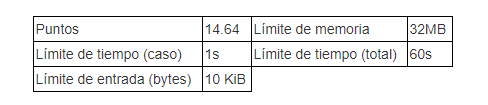
\includegraphics[width=0.7\textwidth]{Abigail/Ejercicio07/Images/1_B.PNG}
    	 	\end{figure} 

            Al final su viaje por cuba, Edgardo se puso a pensar acerca de problemas más interesantes que sus alumnos podrían resolver.

            En esta ocasión tu trabajo es el siguiente: Dadas 2 cadenas A y B, debes de encontrar la subsecuencia común más larga entre ambas cadenas.

            \begin{multicols}{2}
                \noindent\textbf{Entrada} \\ 
                La primera línea contendrá la cadena A. En la segunda linea vendra la cadena B.
                
            \columnbreak
                
                \noindent\textbf{Salida} \\
                La longitud de la subsecuencia común más larga.
            \end{multicols}
            
            \textbf{Ejemplo}    \\
            \begin{figure}[h!]
    	        \centering
    	        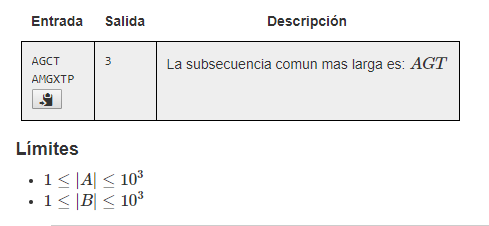
\includegraphics[width=0.5\textwidth]{Abigail/Ejercicio07/Images/1_C.PNG}
    	 	\end{figure} 
    \newpage

        \subsection{Captura del problema aceptado}
            \begin{figure}[h!]
    	        \centering
    	        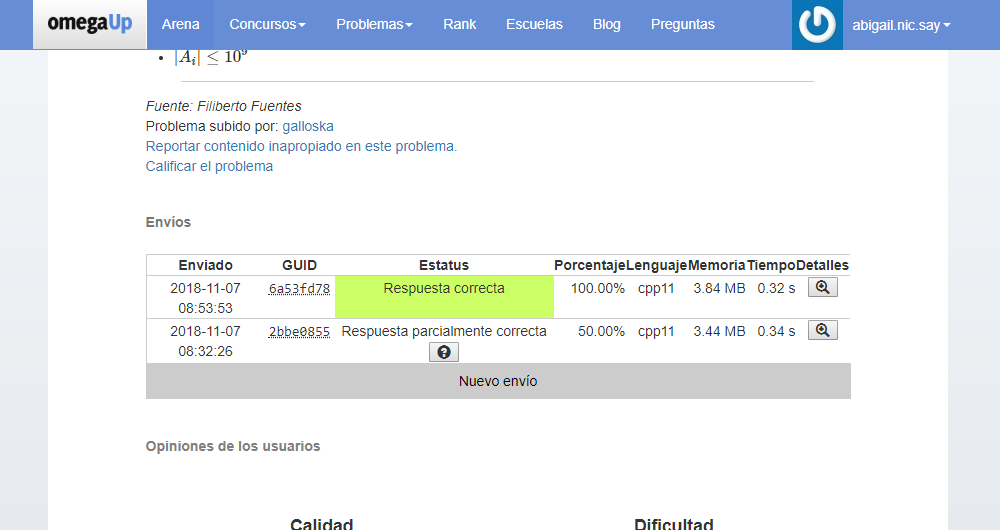
\includegraphics[width=1.0\textwidth]{Abigail/Ejercicio07/Images/1_A.PNG}
    	 	\end{figure} 
        
        \subsection{Explicación}
            La solución bruta para el problema sería el generar todas las subsecuencias de ambas secuencias dadas y encontra susbsecuencia más larga coincidente. 

            Sin embargo, el problema tiene propuedades de subestructura superpuesta y se puede evitar el nuevo cálculo de los mismos subproblemas utilizando la tabulación. 

        \subsection{Código}
        	\inputminted{c++}{Ejercicio07/Code/LCS.c}

%   /////////////////////////////////////////////////////////////
%               Easy Longest Increasing Subsequence
%   ///////////////////////////////////////////////////////////
\newpage
  \section{Easy Longest Increasing Subsequence}
  
    \subsection{Redacción}
        \begin{figure}[h!]
	        \centering
	        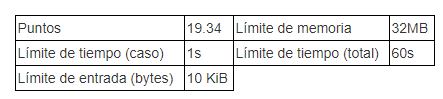
\includegraphics[width=0.7\textwidth]{Abigail/Ejercicio06/Images/2_B.PNG}
	 	\end{figure} 

        Tienes dos amigos \textbf{A} ambos quieres regalarles varios números enteros como obsequio. A tu primera amigo quieres regalarle $C_{1}$ enteros y a tu segundo amigo quieres regalarle $C_{2}$ enteros. No satisfecho con eso, también quieres que todos los regalos únicos, lo cual implica que no podrás regalar el mismo entero a ambos de tus amigos.
        
        Además de eso, a tu primer amigo no le gustan los enteros que son divisibles por el número primo $X$. A tu segundo amigo no le gustan los enteros que son divisibles por el número primo $Y$. Por su puesto, tu no le regalarás a tus amigos números que no les gusten.
        
        Tu objetivo es encontrar el mínimo número $V$, de tal modo que puedas dar los regalos a tus amigos utilizando únicamente enteros del conjunto $1$, $2$, $3$, ..., $V$. Por supuesto, tú podrías decidir no regalar algunos enteros de ese conjunto.
        
        Un número entero positivo mayor a 1 es llamado primo si no tiene divisores enteros positivos además del 1 y el mismo.
        
        \begin{multicols}{2}
            \noindent\textbf{Entrada} \\ 
            Una línea que contiene cuatro enteros positivos $C_{1}$, $C_{2}$, $X$, $Y$.     \\
            Se garantiza que $X$ y $Y$ son números primos.
            
        \columnbreak
            
            \noindent\textbf{Salida} \\
            Una línea. Un entero que representa la respuesta al problema.
        \end{multicols}
        
        \textbf{Ejemplo}    \\
        \begin{figure}[h!]
	        \centering
	        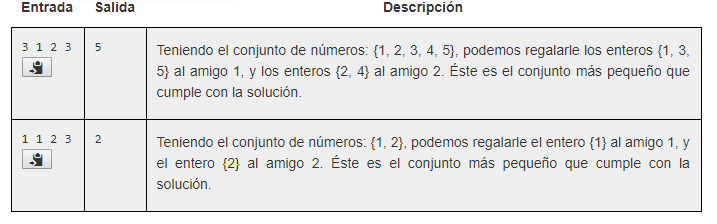
\includegraphics[width=0.9\textwidth]{Abigail/Ejercicio06/Images/2_C.PNG}
	 	\end{figure} 
	 	
\newpage

    \subsection{Captura del problema aceptado}
        \begin{figure}[h!]
	        \centering
	        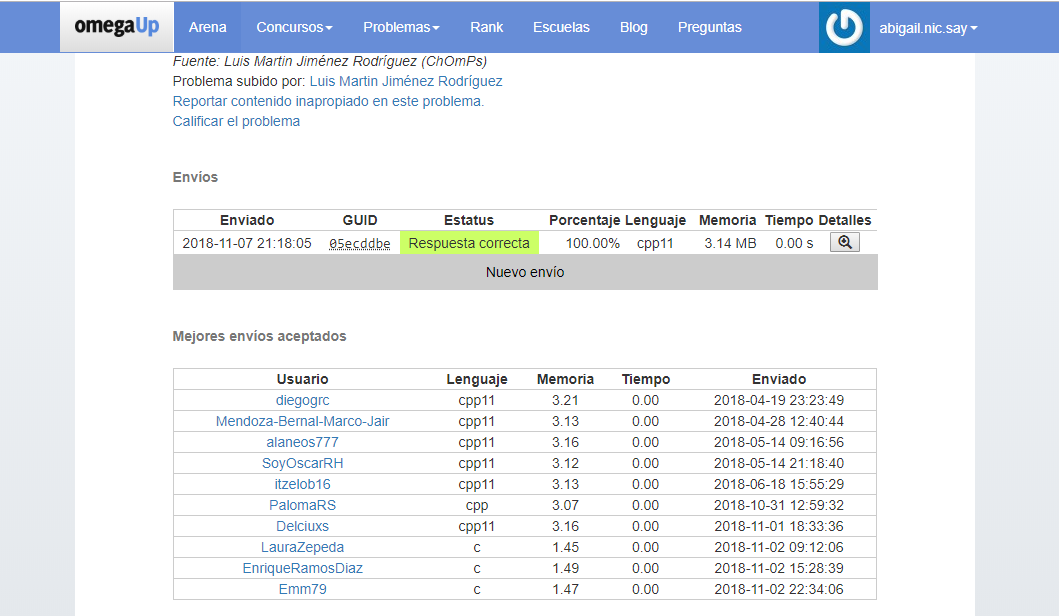
\includegraphics[width=1.0\textwidth]{Abigail/Ejercicio06/Images/2_A.PNG}
	 	\end{figure} 
      
    \subsection{Explicación}
    La solución \textbf{Bruta}, sería hacer un ciclo que valide cada elemento que tenemos e ir viendo cuales cumplen con las características, en el peor de los casos la complejidad es $O(n)$.
    
    La solución implementada se explica a continuación, con complejidad $O\left(log2[C_{1}+C_{2}]\right)$.:
    
        \begin{itemize}
            \item Números no divisibles en el conjunto  \\
            
            Se busca el número de elementos que no son divisibles entre $X$ ó/y $Y$. 
            
            \item Revisar si se pueden regalar
            
            Se descartan regalos entre los amigos para no darles los mismos. 
            
            \item Revisar si los regalos no superan los regalos disponibles.
        \end{itemize}
\newpage
    \subsection{Código}
    	\inputminted{c++}{Code/2.c}

%   /////////////////////////////////////////////////////////////
%               KNAPSACK - The Knapsack Problem
%   ///////////////////////////////////////////////////////////
\newpage
  \section{KNAPSACK - The Knapsack Problem}
  
    \subsection{Redacción}
        El famoso problema de la mochila. Estás empacando para unas vacaciones a lado del mar y solo llevas una bolsa con capacidad S $(1<=$ S $<=2000)$. También tiene N $(1<=$ N $<=2000)$ elementos que puede llevar consigo al lado del mar. Lamentablemente, no puede colocarlos todos en la mochila, por lo que tendrá que elegir. Para cada artículo se le da su tamaño y su valor. Se desea maximizar el valor total de todos los artículos que va a traer. ¿Cuál es este valor total máximo?

        \begin{multicols}{2}
            \noindent\textbf{Entrada} \\ 
            En la primera línea te dan S y N. Las líneas N siguen con dos enteros en cada línea que describe uno de sus elementos. El primer número es el tamaño del artículo y el siguiente es el valor del artículo.
            
        \columnbreak
            
            \noindent\textbf{Salida} \\
            Debe generar un único enero en uno como: el valor máximo total de la mejor selección de elementos para su viaje.
        \end{multicols}
        
        \textbf{Ejemplo}    \\
        \begin{figure}[h!]
            \centering
            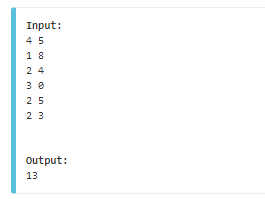
\includegraphics[width=0.9\textwidth]{Abigail/Ejercicio07/Images/2_C.PNG}
        \end{figure} 
        
\newpage

    \subsection{Captura del problema aceptado}
        \begin{figure}[h!]
            \centering
            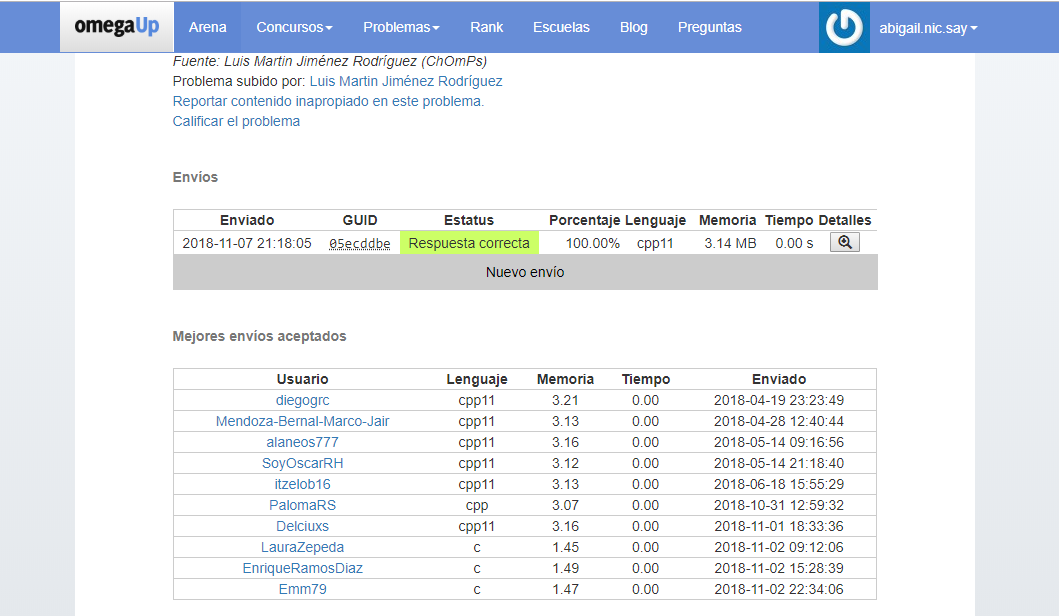
\includegraphics[width=1.0\textwidth]{Abigail/Ejercicio06/Images/2_A.PNG}
        \end{figure} 
      
    \subsection{Explicación}
    La solución \textbf{Bruta}, sería hacer un ciclo que valide cada elemento que tenemos e ir viendo cuales cumplen con las características, en el peor de los casos la complejidad es $O(n)$.
    
    La solución implementada se explica a continuación, con complejidad $O\left(log2[C_{1}+C_{2}]\right)$.:
    
        \begin{itemize}
            \item Números no divisibles en el conjunto  \\
            
            Se busca el número de elementos que no son divisibles entre $X$ ó/y $Y$. 
            
            \item Revisar si se pueden regalar
            
            Se descartan regalos entre los amigos para no darles los mismos. 
            
            \item Revisar si los regalos no superan los regalos disponibles.
        \end{itemize}
\newpage
    \subsection{Código}
        \inputminted{c++}{Code/2.c}

\end{document}